\section{Audio Captcha Services}
\label{sec:services}

In this section we provide an overview of the captcha services that we found in the wild
that also provide audio captchas. We provide information on the characteristics of the audio challenges, as
well as some details about extra steps needed to avoid safeguards deployed by certain services for 
detecting automated attacks.

%\jason{What are the checks deployed by each service? How do we bypass them? E.g., highlighting boxes etc.}

\begin{table}[t]
\centering
\caption{Description and characteristics of the captcha services that we evaluate.}
\begin{tabular}{lccc}
\toprule
\textbf{Service}& \textbf{Dictionary}& \textbf{Length} & \textbf{Noise} \\
\hline
%Recaptcha v1 & Digits & \jason{?} & None \\
Recaptcha v2.0 & Digits & 5 & None \\
\rowcolor{Gray}
Recaptcha v2.1 & Digits & 10 & None \\
Apple & Numbers (10-99) & 3-5 & Moderate\\
\rowcolor{Gray}
BotDetect & Digits, Alphabet & 1-13 & High \\
Captchas.net & NATO alphabet & 6 & None \\
\rowcolor{Gray}
Microsoft Live & Words & 5-7 & Moderate \\
Securimage & Digits, Alphabet & 6 & High \\
\rowcolor{Gray}
Telerik & Digits, NATO & 5 & None \\
\bottomrule
\end{tabular}
\label{tab:services}
\end{table}

\begin{figure}[tp]
%\begin{subfigure}{0.3\textwidth}
%        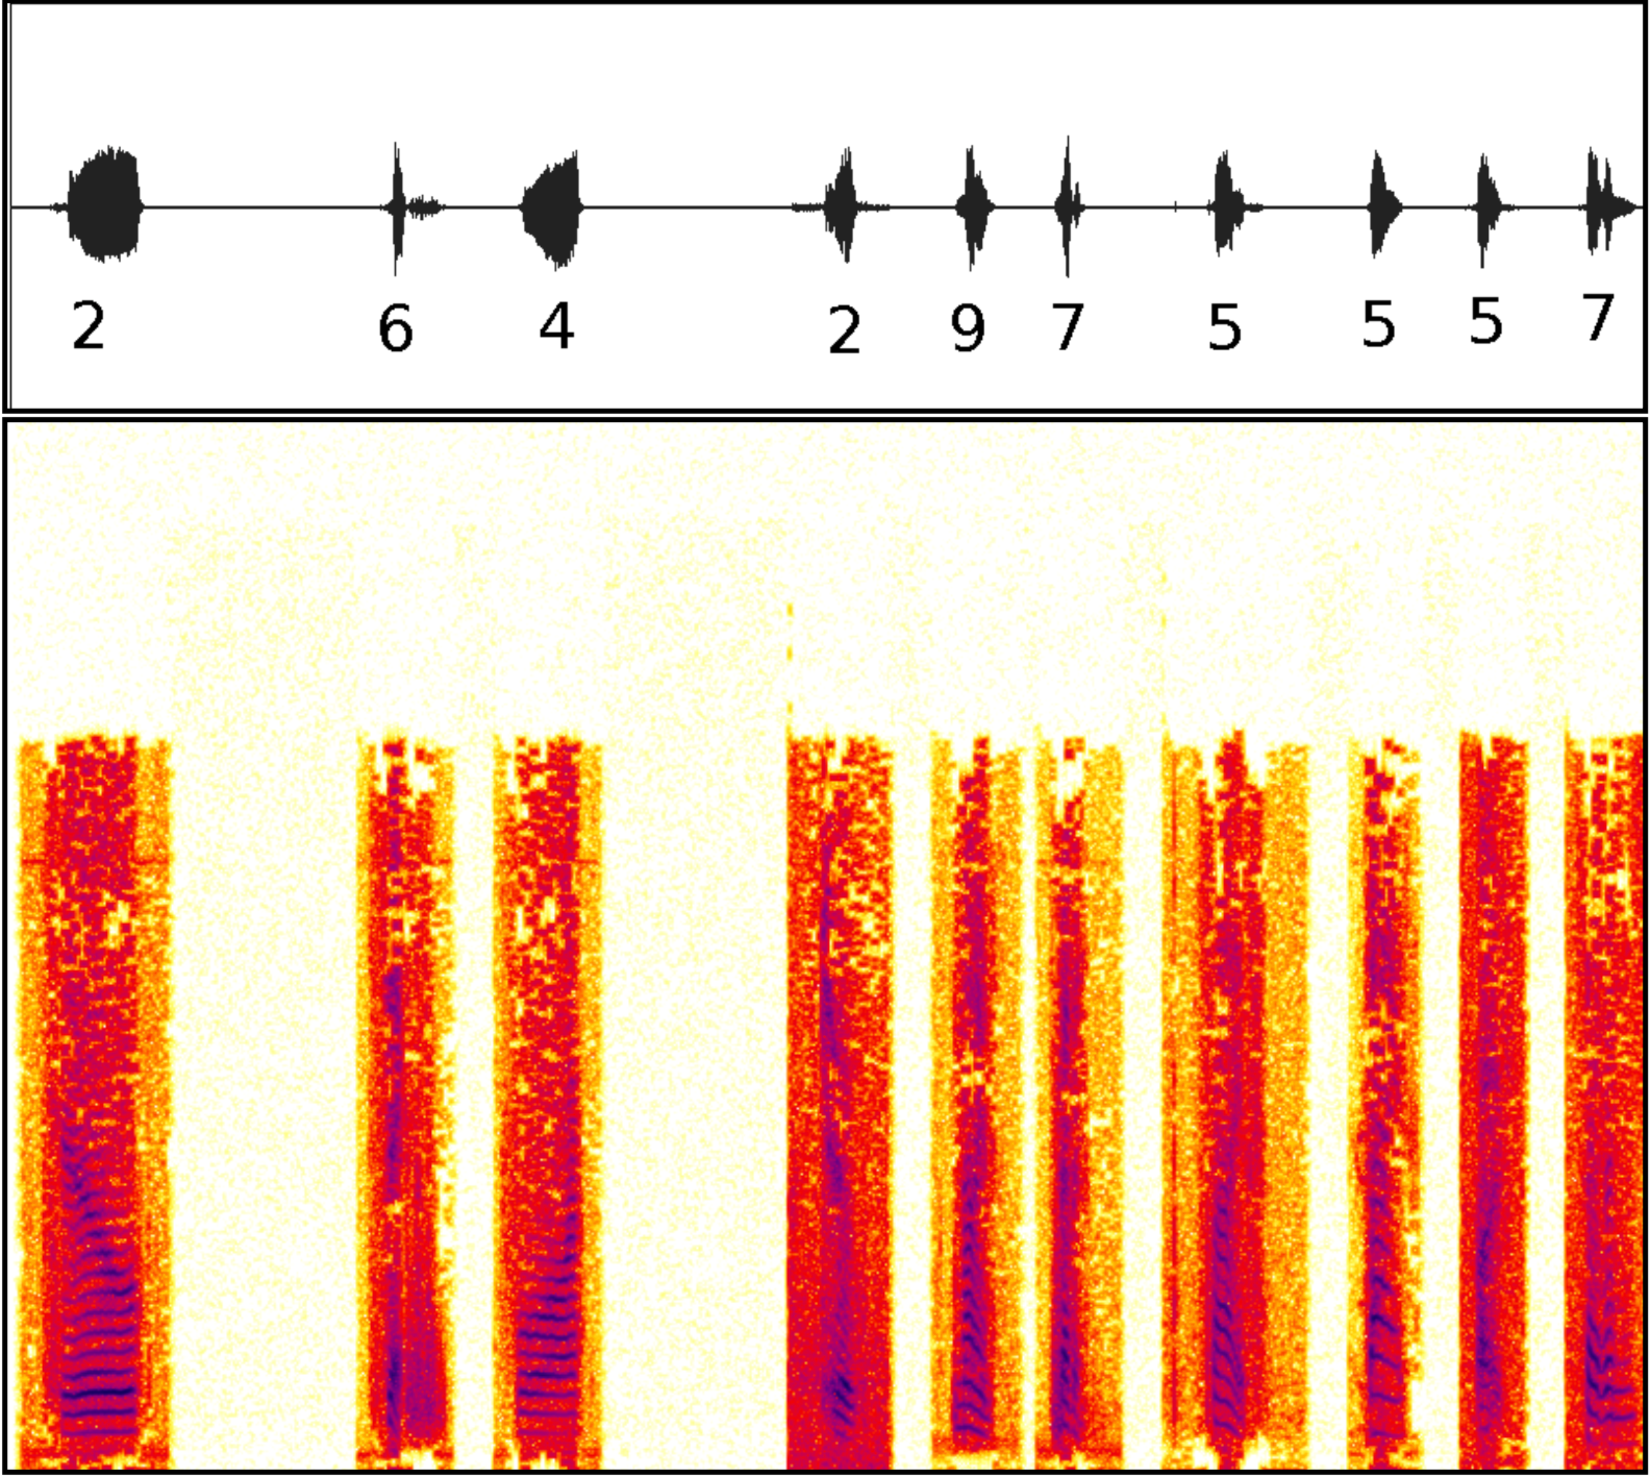
\includegraphics[width=\textwidth]{figures/recaptcha1.pdf}
%        \caption{\re v1}
%        \label{fig:recaptcha1}
%\end{subfigure} %\hspace{0.03\textwidth}
\begin{subfigure}{0.23\textwidth}
        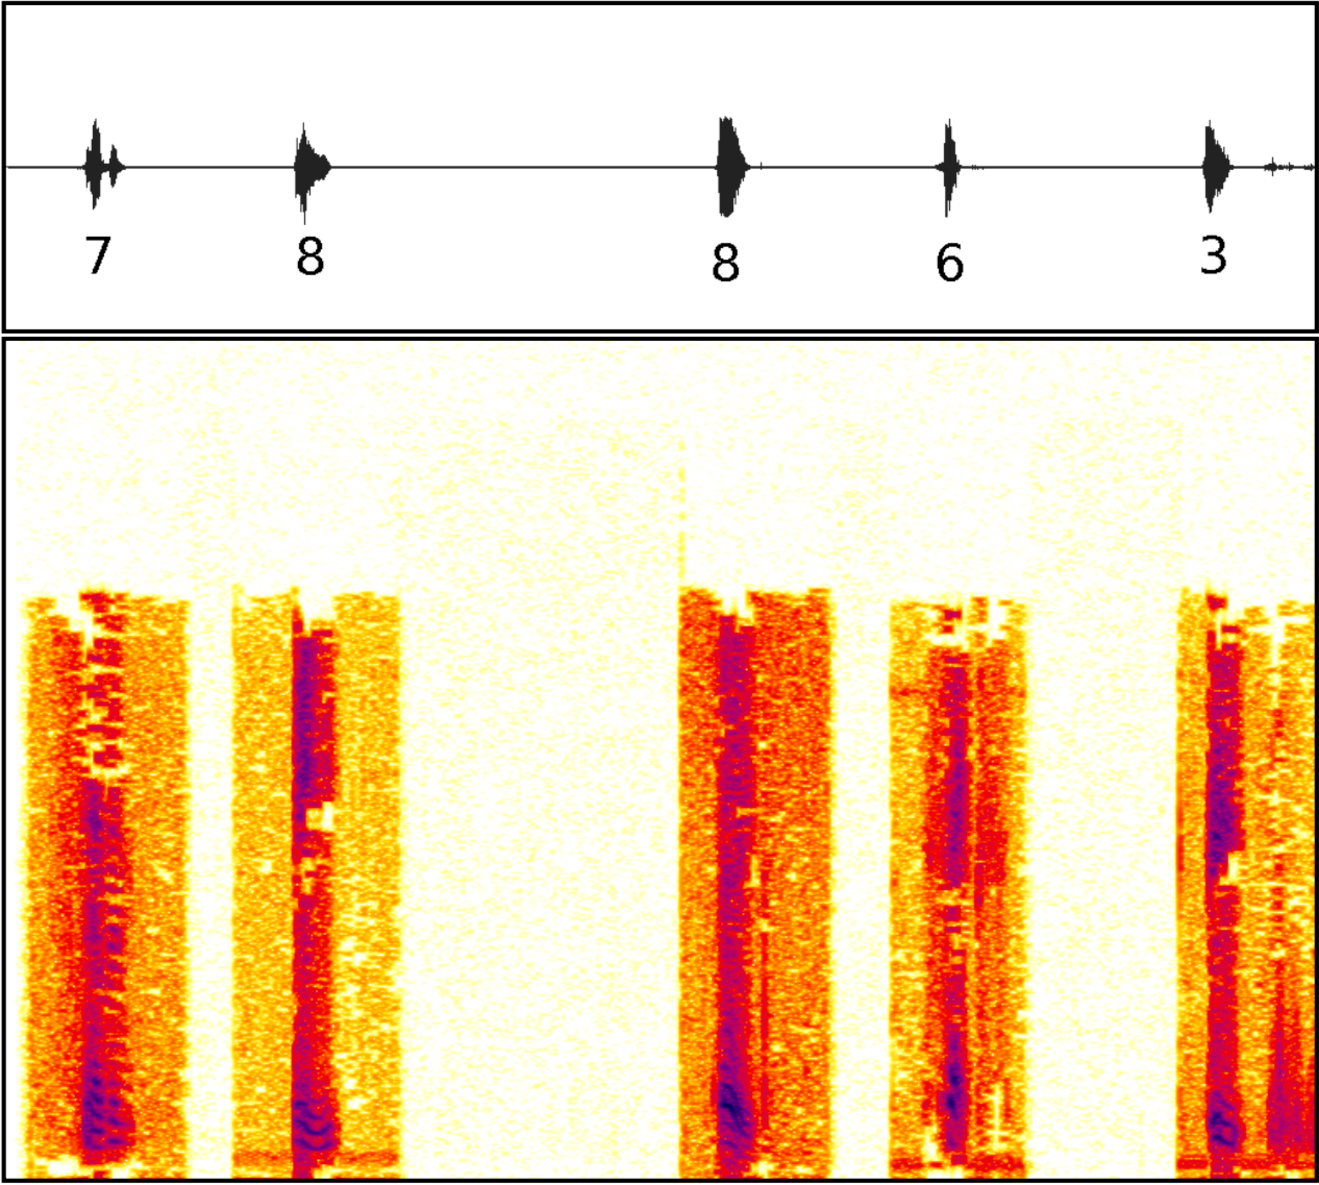
\includegraphics[width=\textwidth]{figures/recaptcha2a.pdf}
        \caption{\re v2.0}
        \label{fig:recaptcha2a}
\end{subfigure}\hspace{0.01\textwidth}
\begin{subfigure}{0.23\textwidth}
        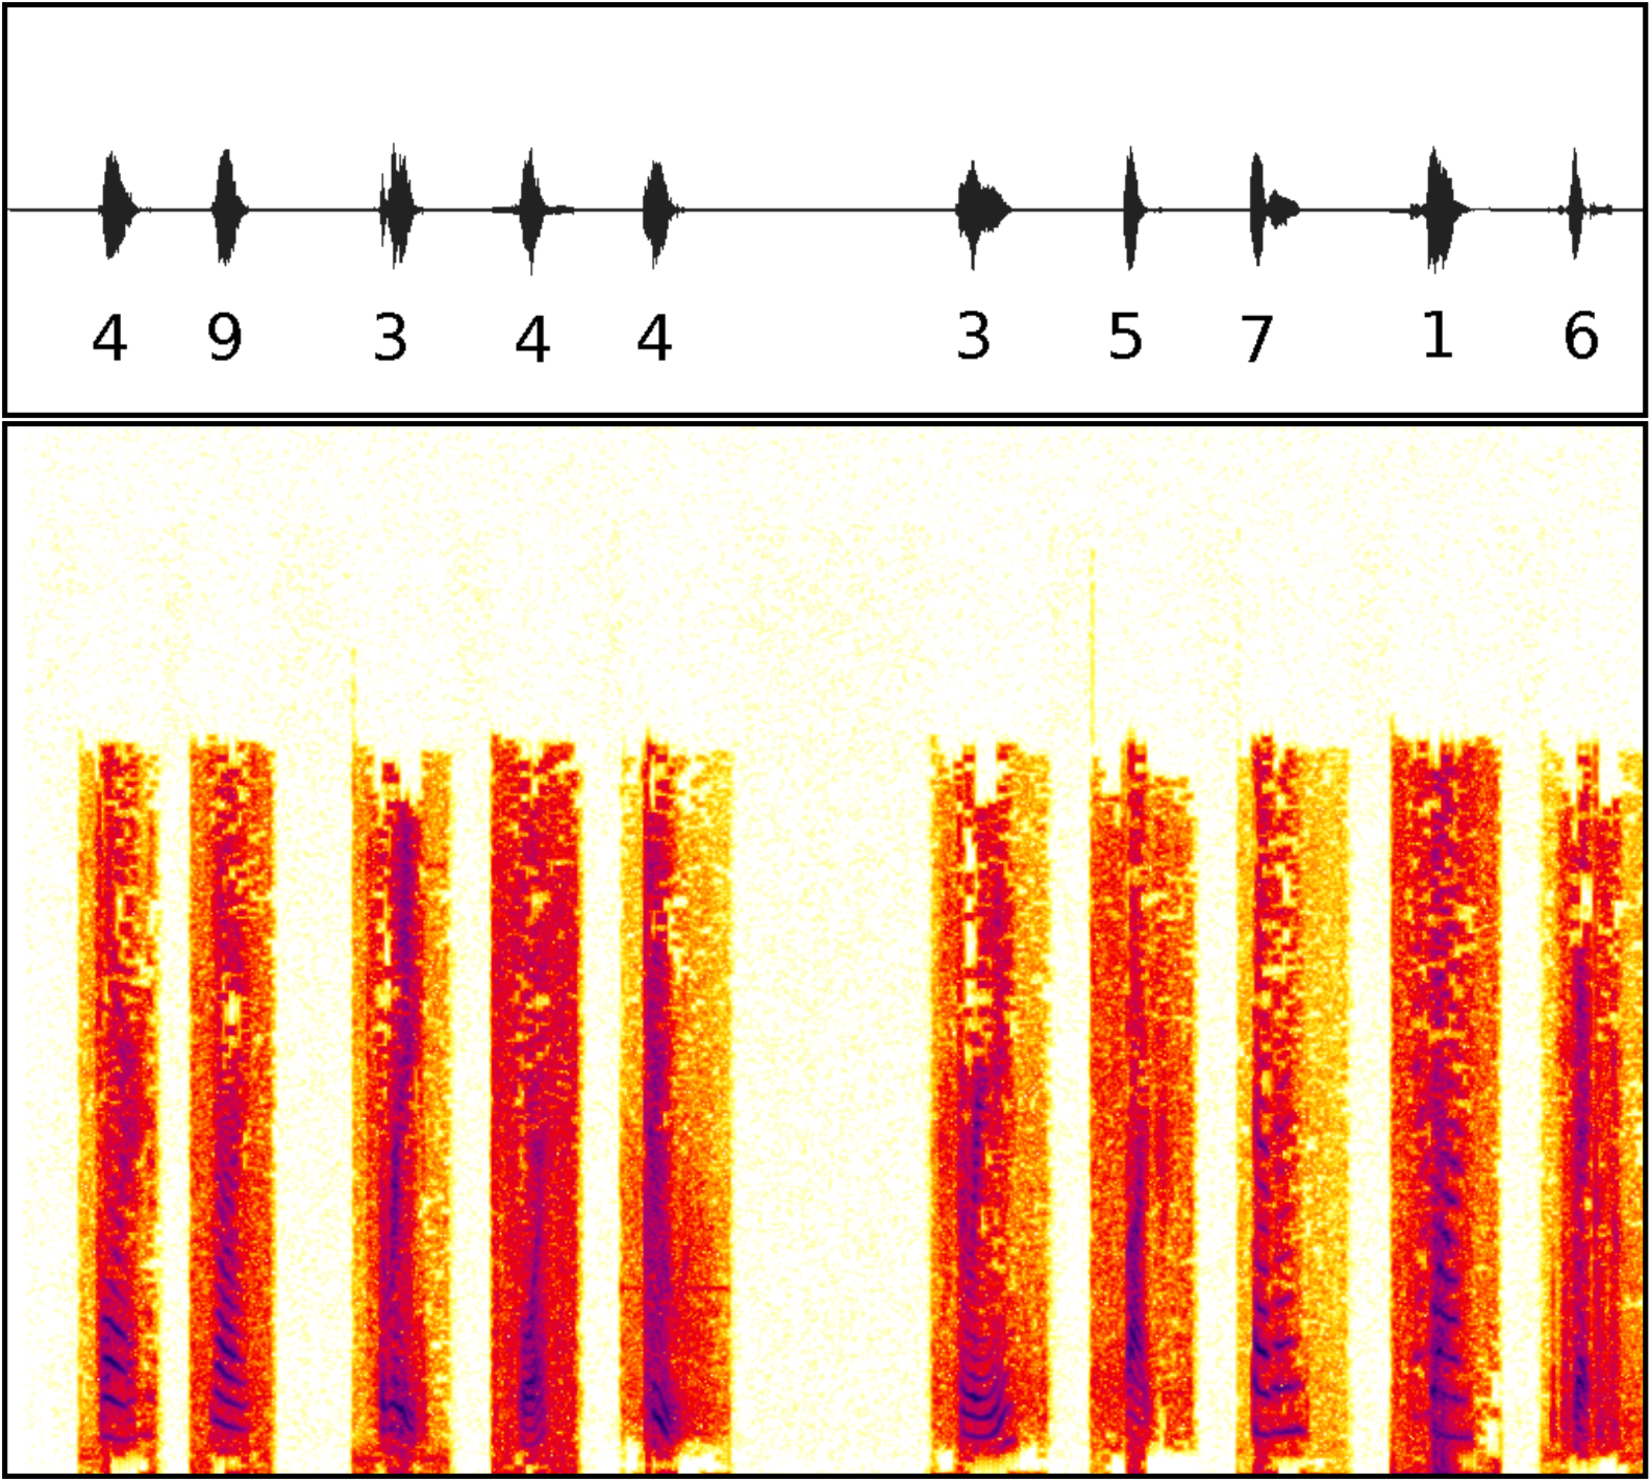
\includegraphics[width=\textwidth]{figures/recaptcha2b.pdf}
        \caption{\re v2.1}
        \label{fig:recaptcha2b}
\end{subfigure}
\caption{Waveforms and corresponding spectrograms for a representative sample challenge from the different versions of Google \re.}
\label{fig:examples}
\end{figure}

\begin{figure*}[tp]
\begin{subfigure}{0.3\textwidth}
        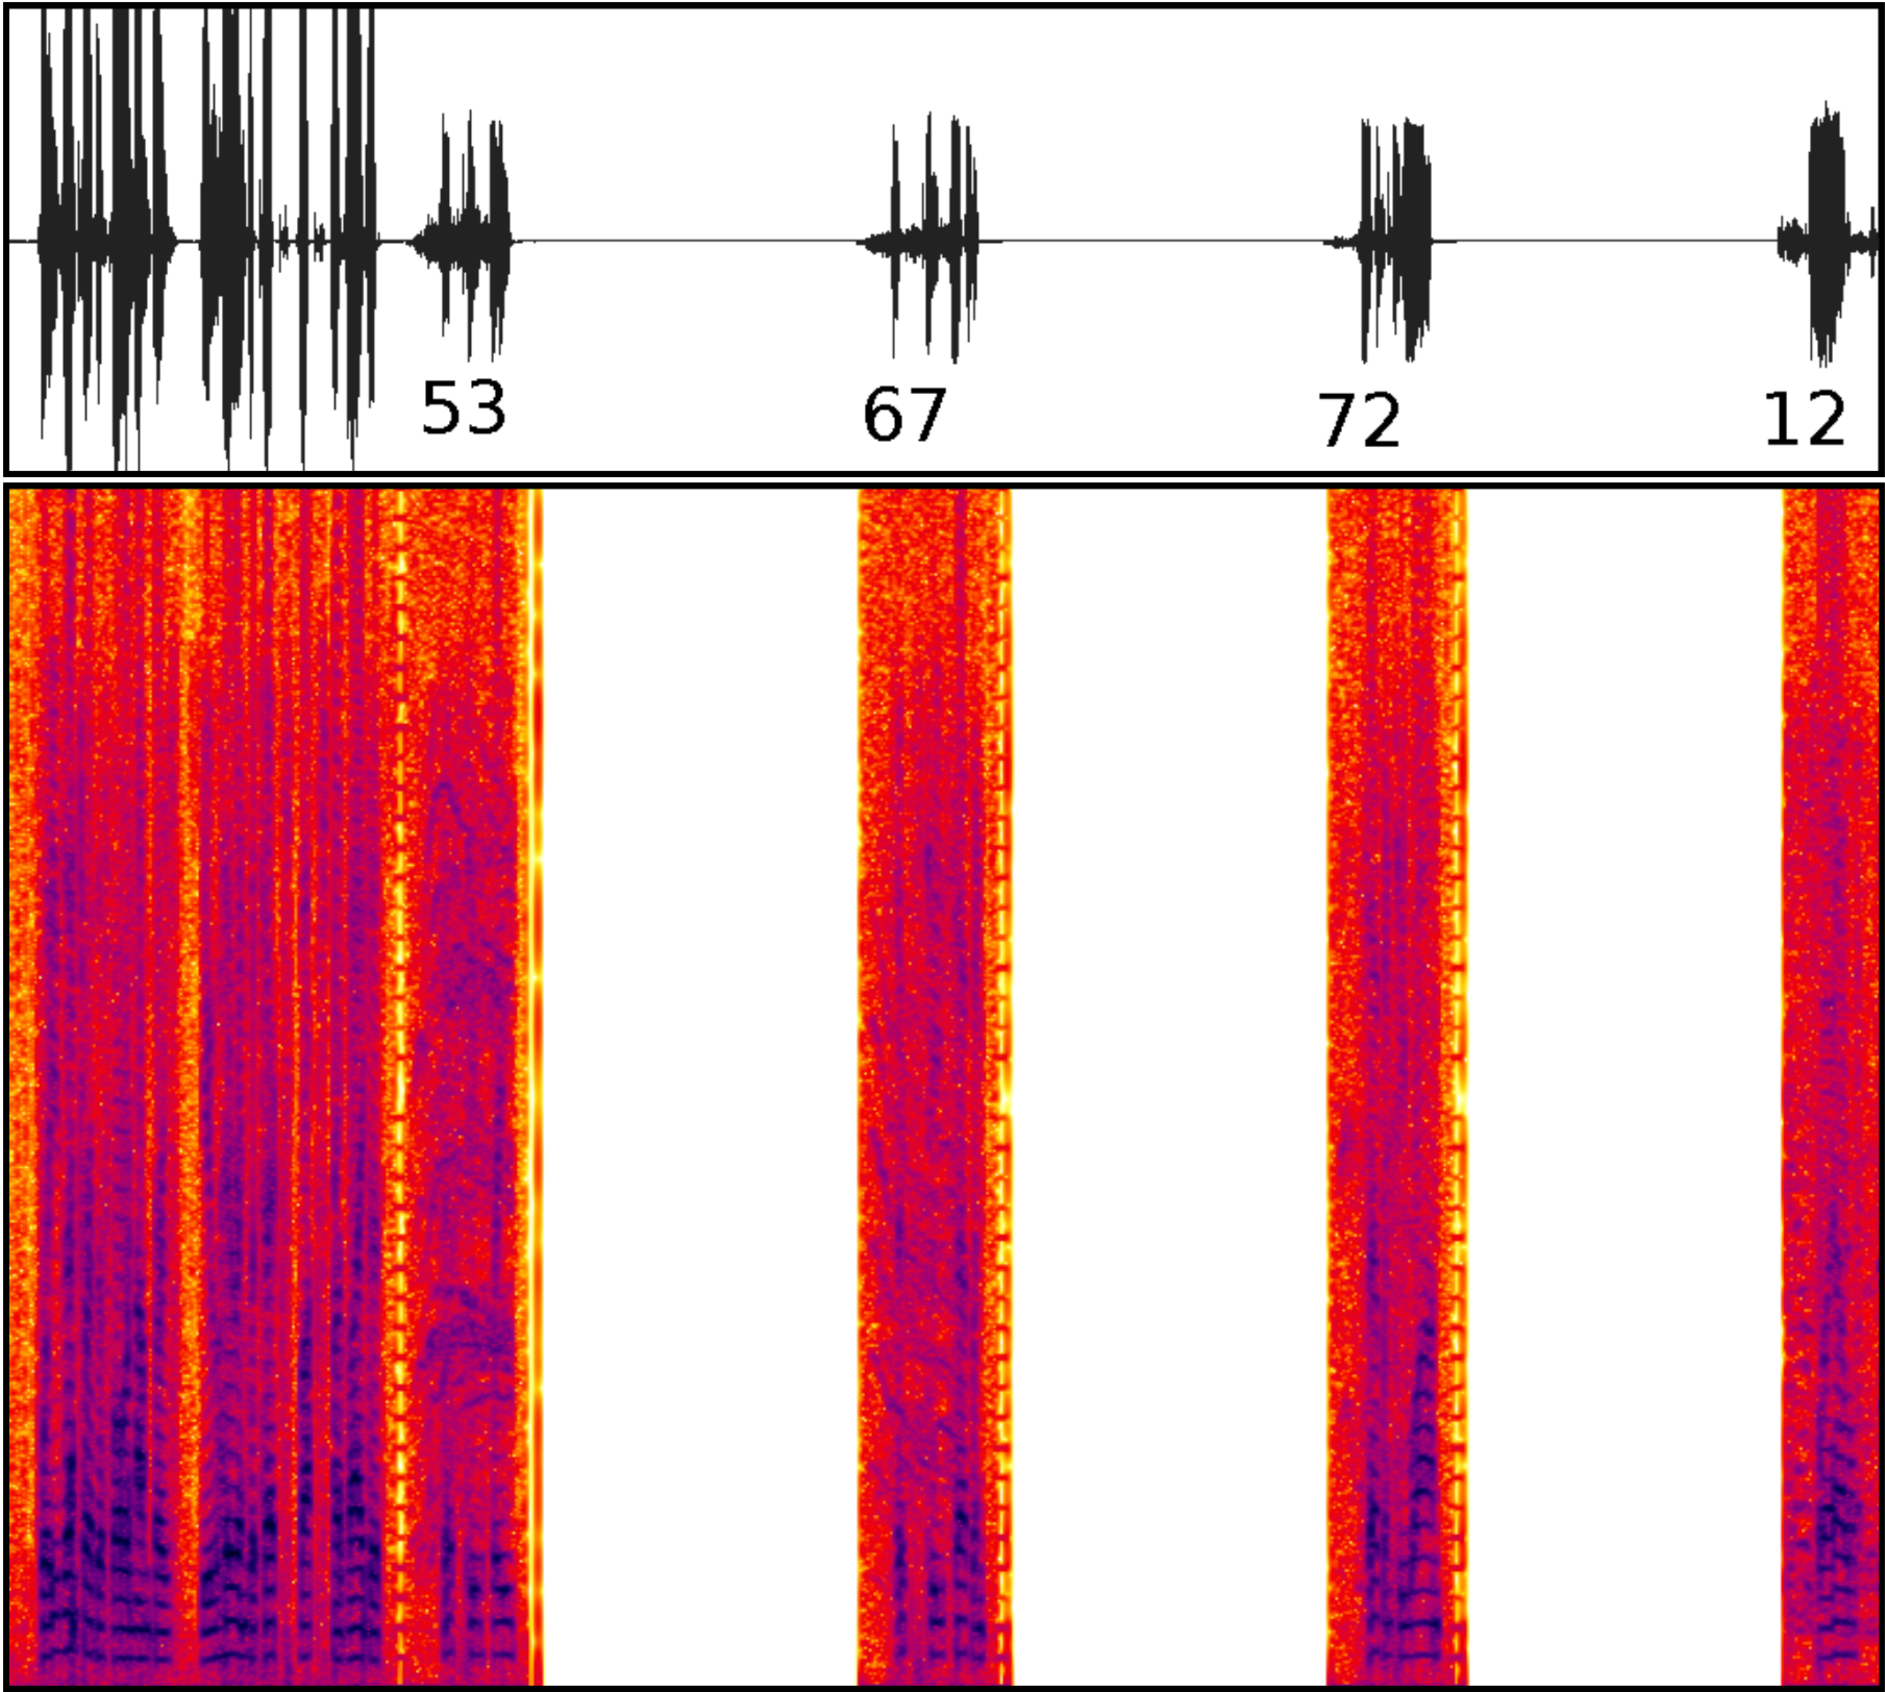
\includegraphics[width=\textwidth]{figures/apple.pdf}
        \caption{Apple}
        \label{fig:apple}
\end{subfigure} \hspace{0.03\textwidth}
\begin{subfigure}{0.3\textwidth}
        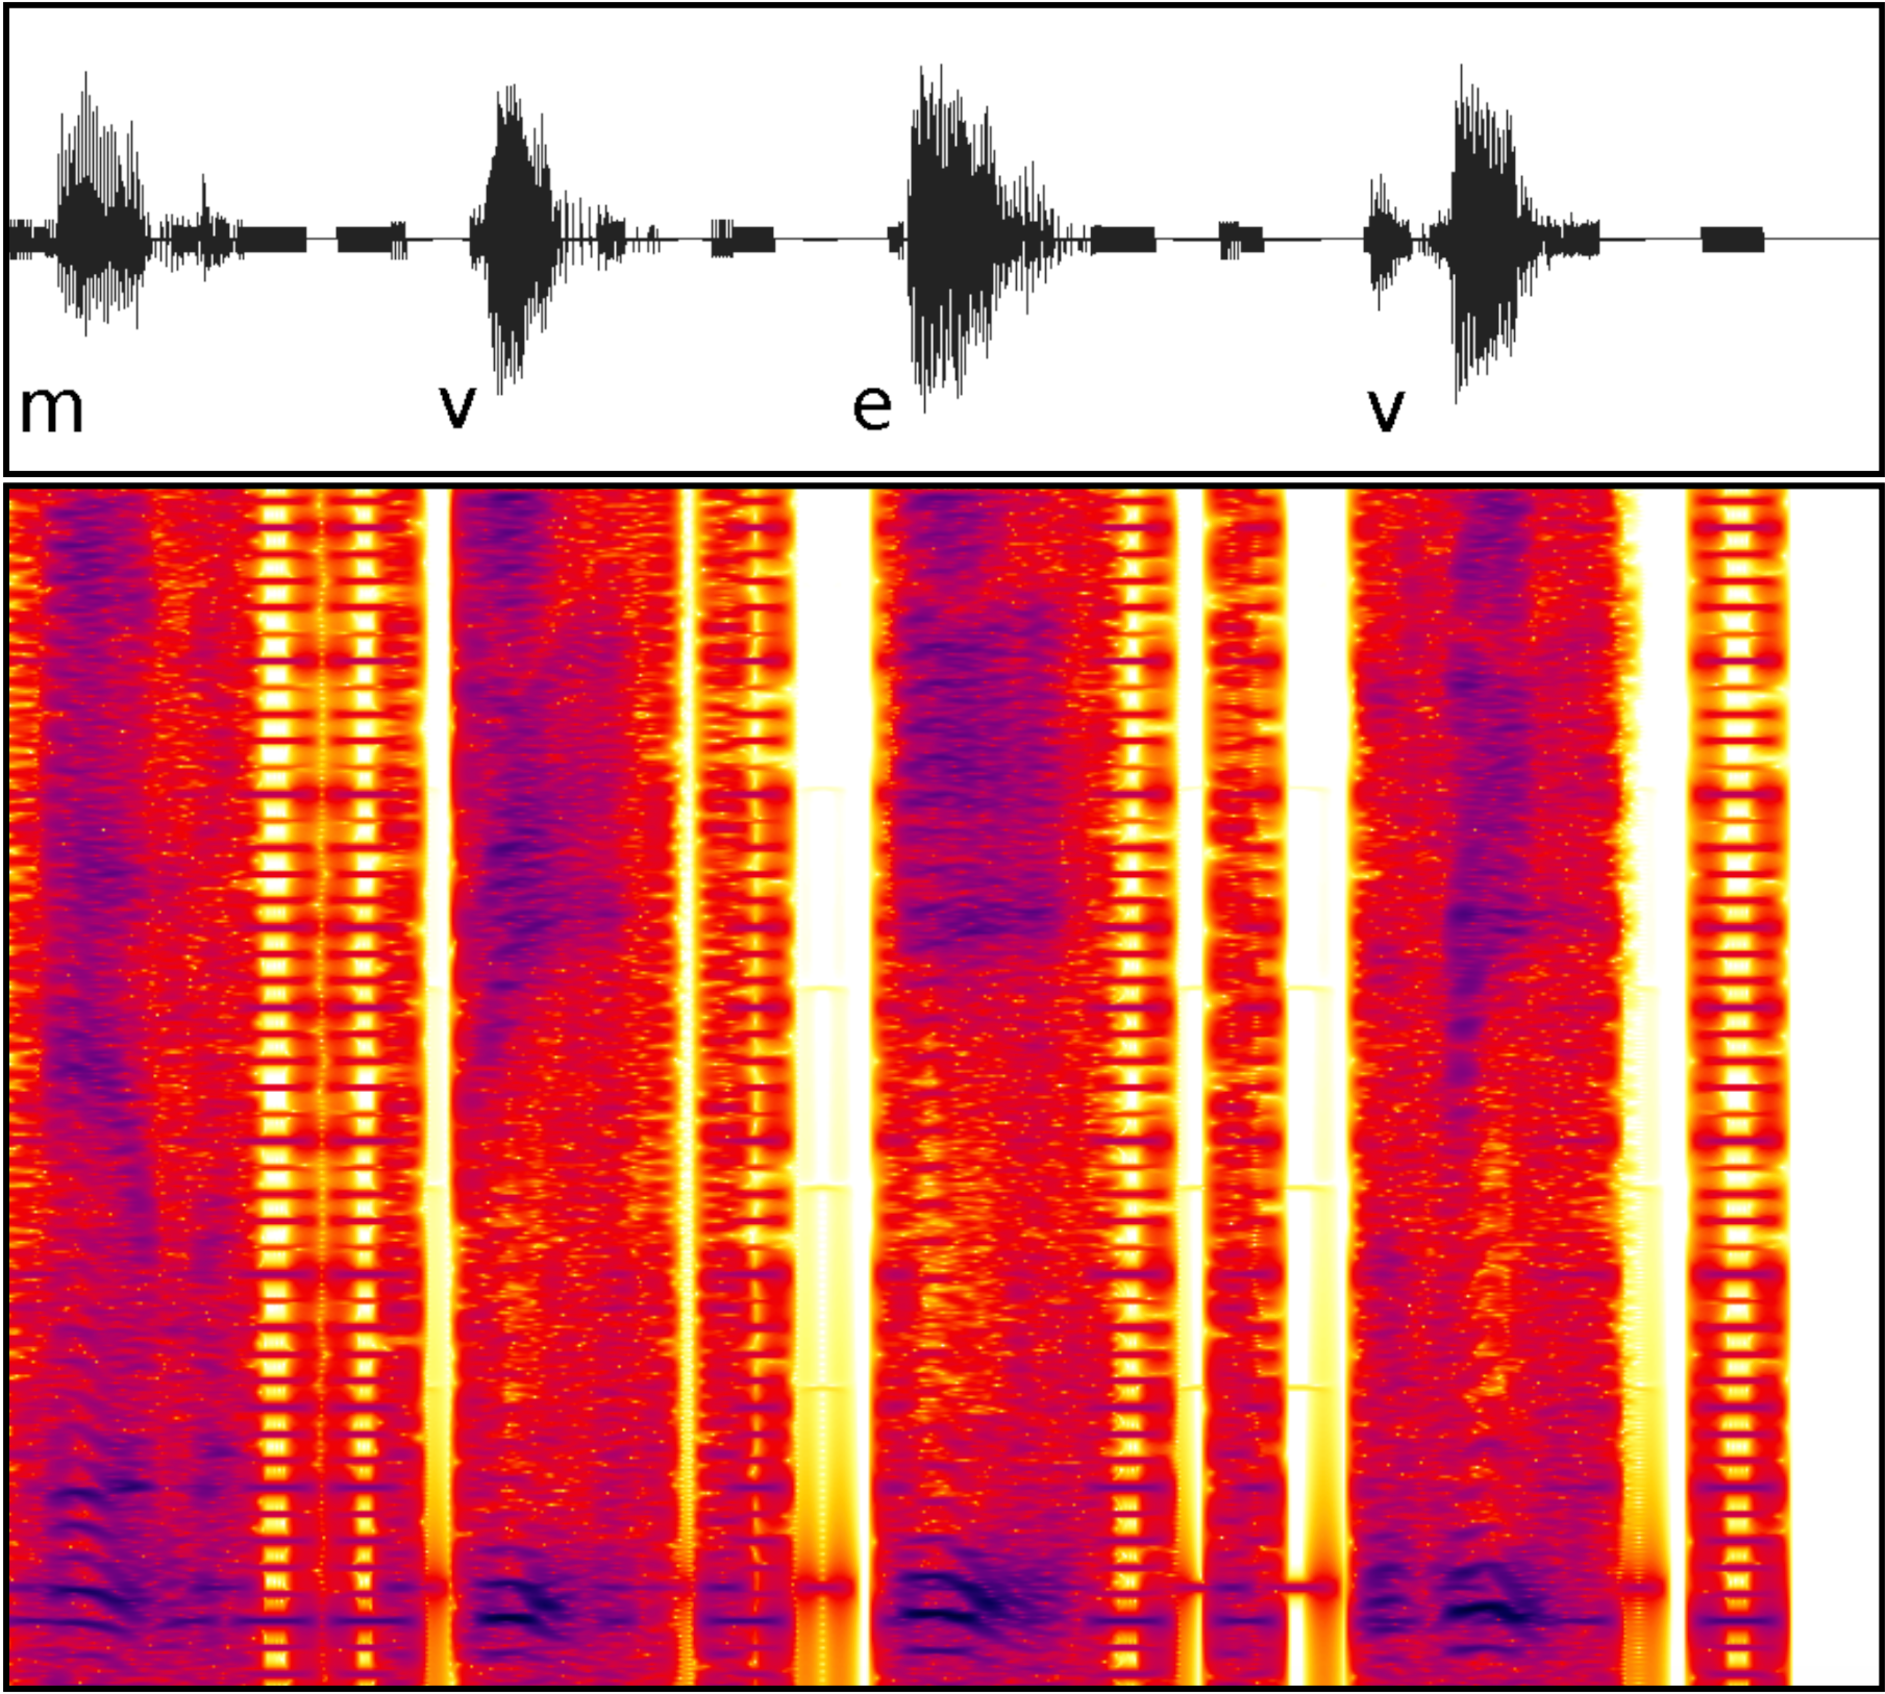
\includegraphics[width=\textwidth]{figures/botdetect.pdf}
        \caption{BotDetect}
        \label{fig:botdetect}
\end{subfigure}\hspace{0.03\textwidth}
\begin{subfigure}{0.3\textwidth}
        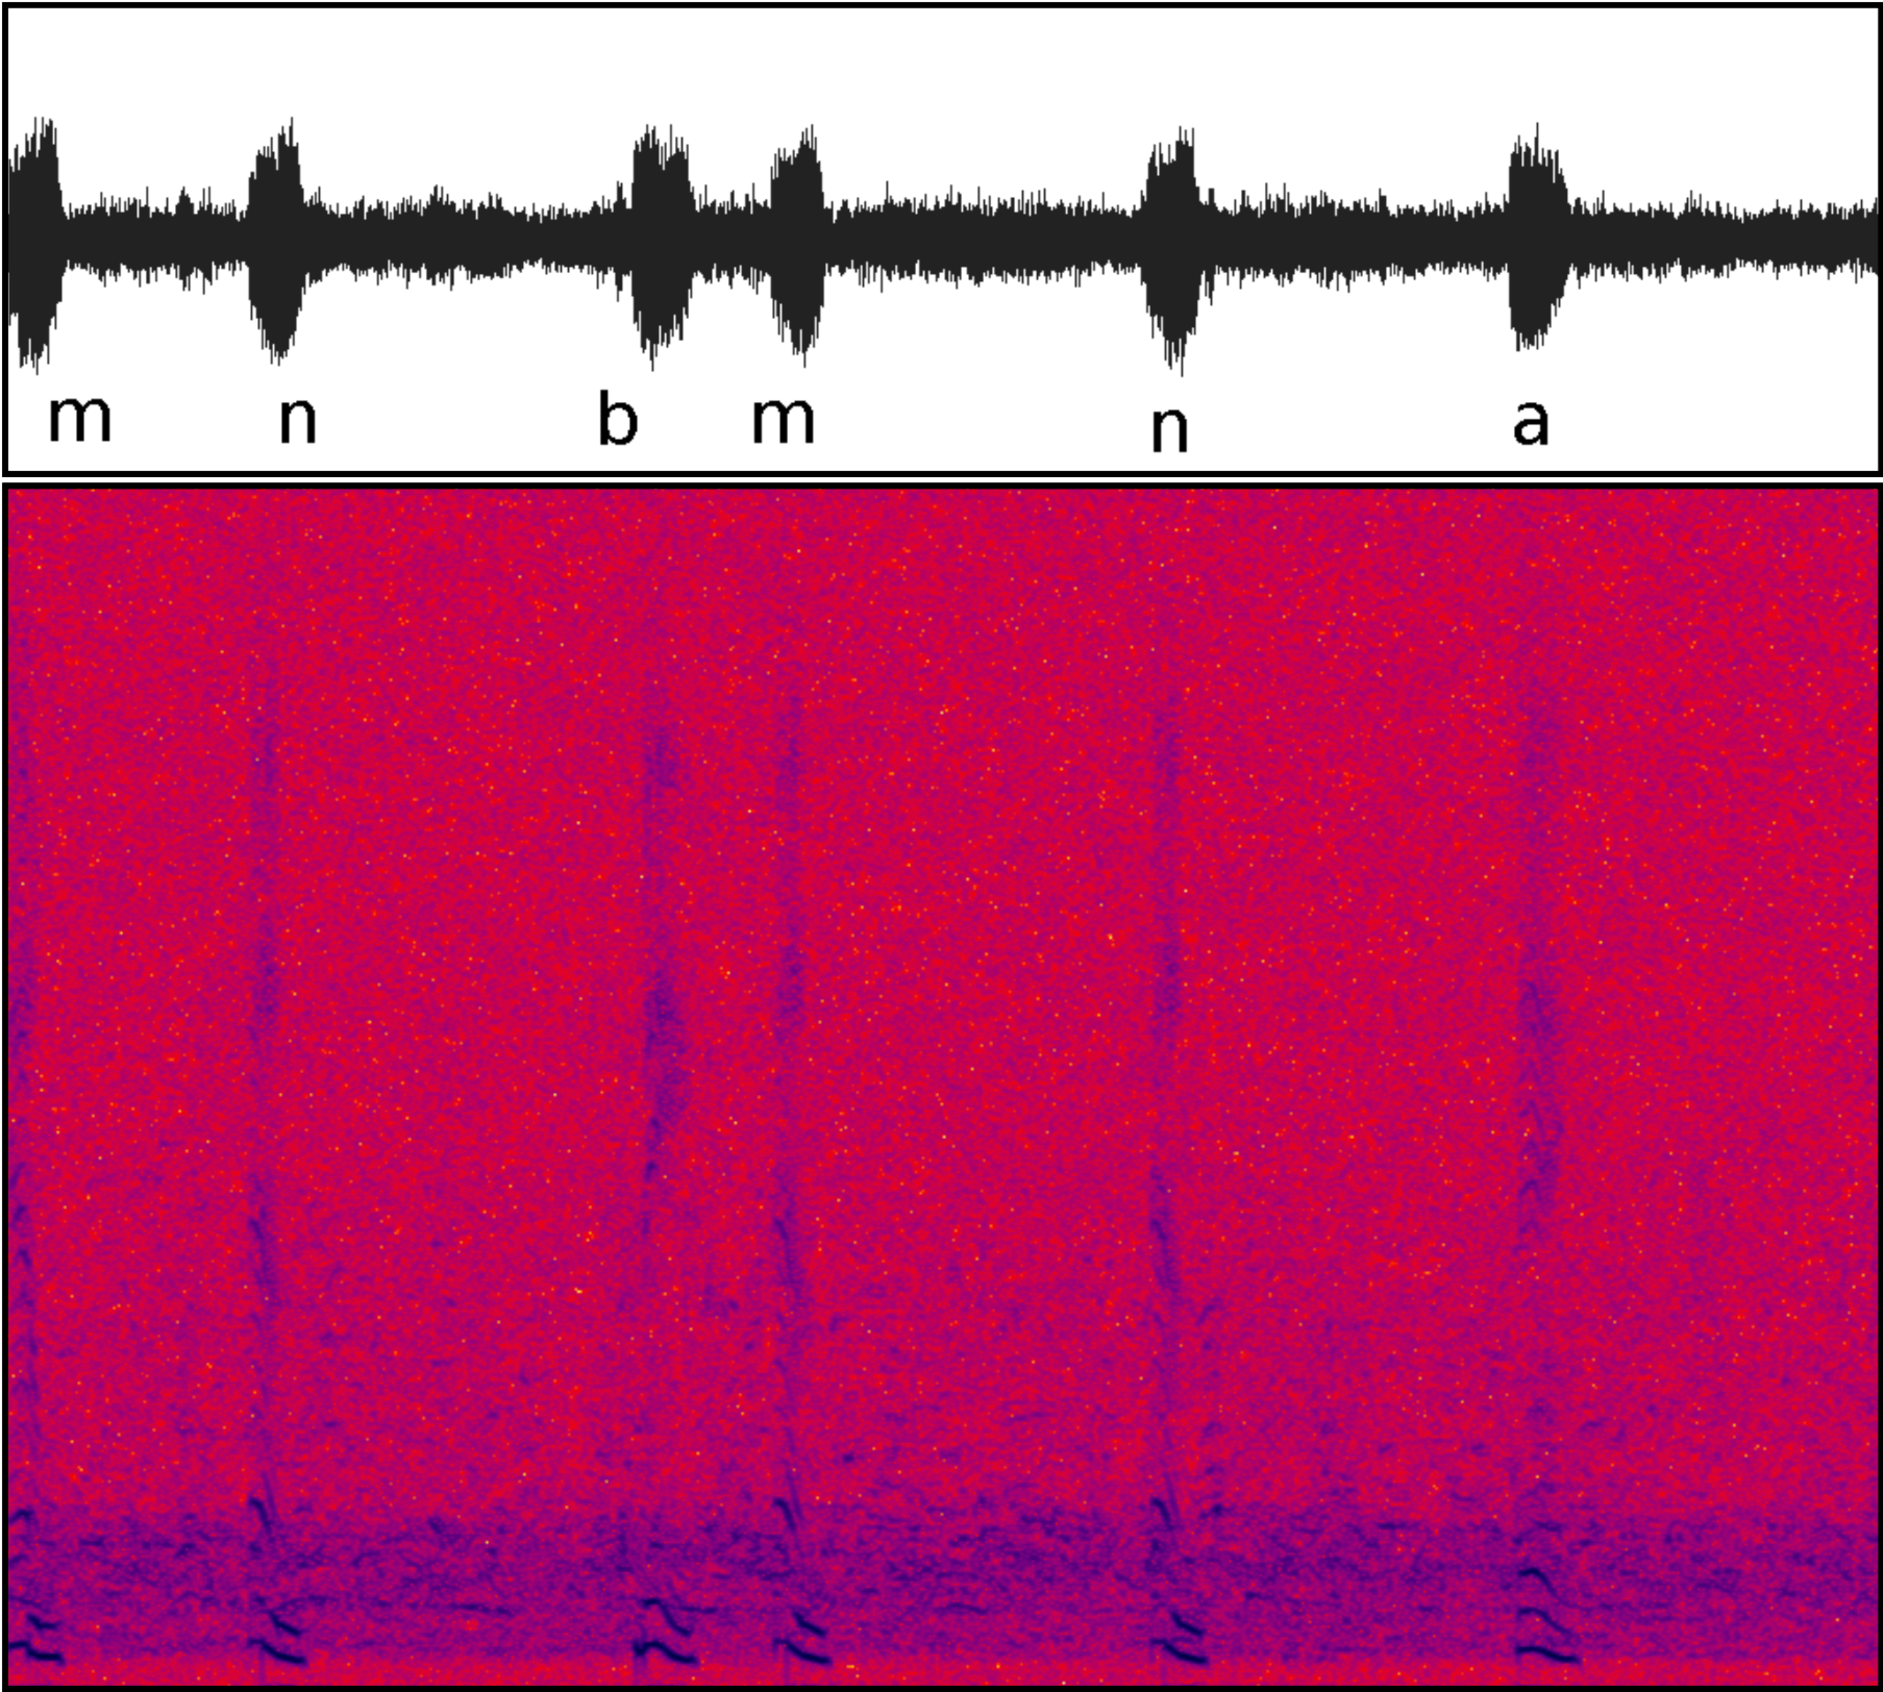
\includegraphics[width=\textwidth]{figures/captchas.pdf}
        \caption{Captchas.net}
        \label{fig:captchas}
\end{subfigure} \\
\begin{subfigure}{0.3\textwidth}
        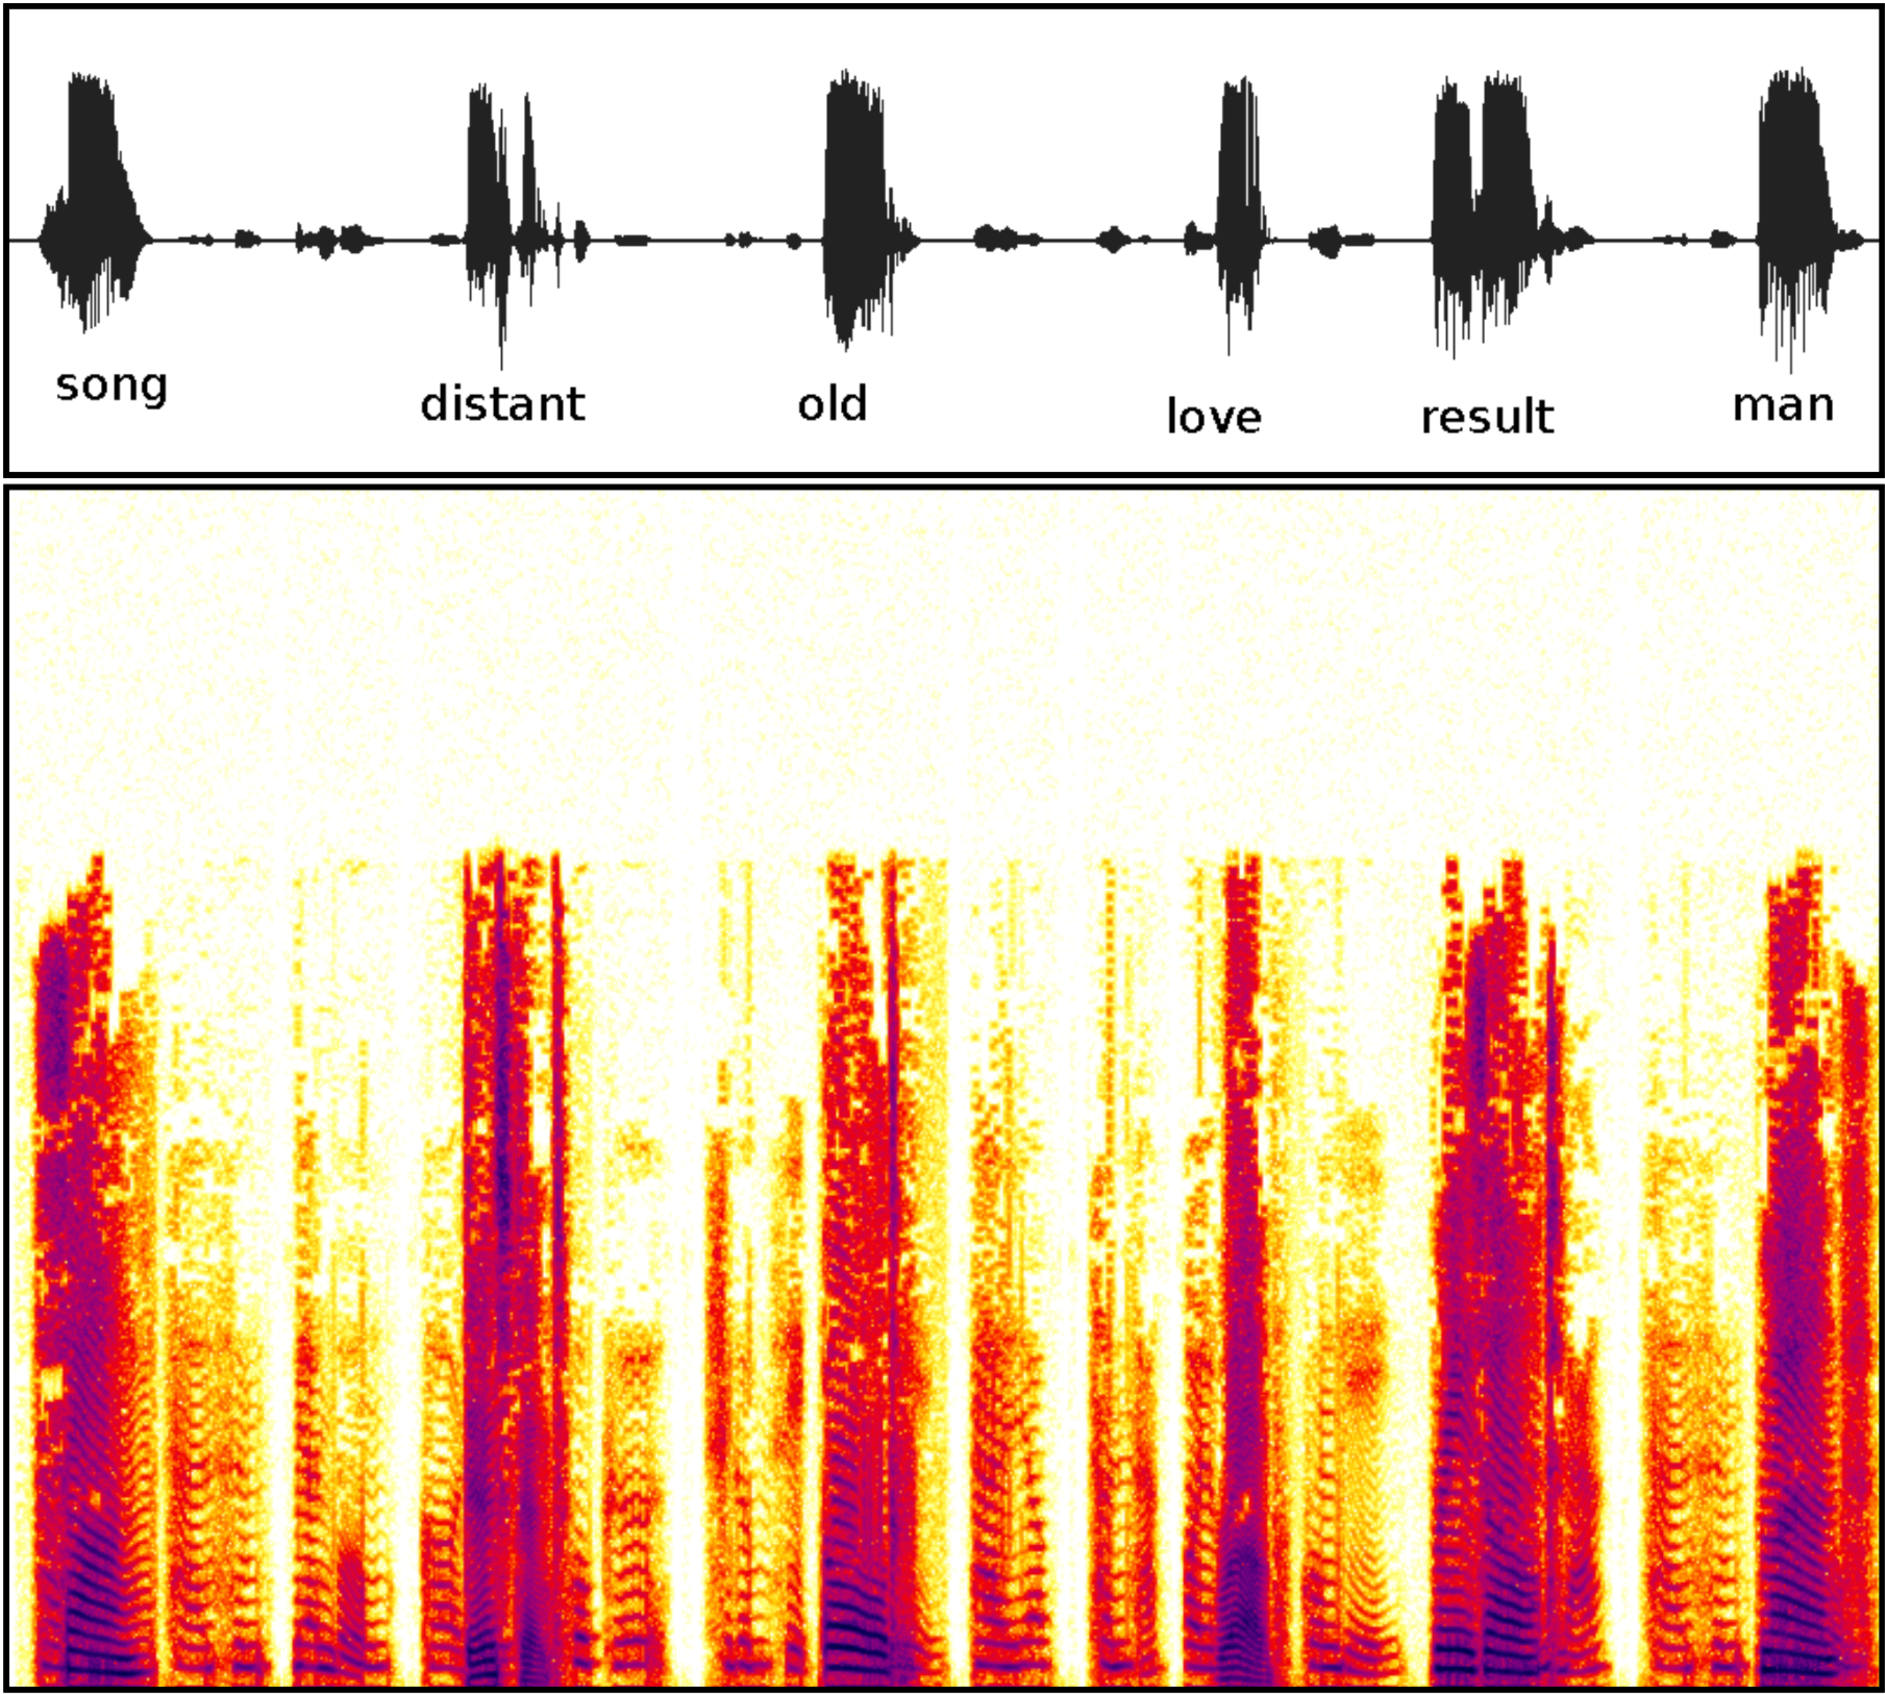
\includegraphics[width=\textwidth]{figures/live.pdf}
        \caption{Microsoft Live}
        \label{fig:live}
\end{subfigure}\hspace{0.03\textwidth} 
\begin{subfigure}{0.3\textwidth}
        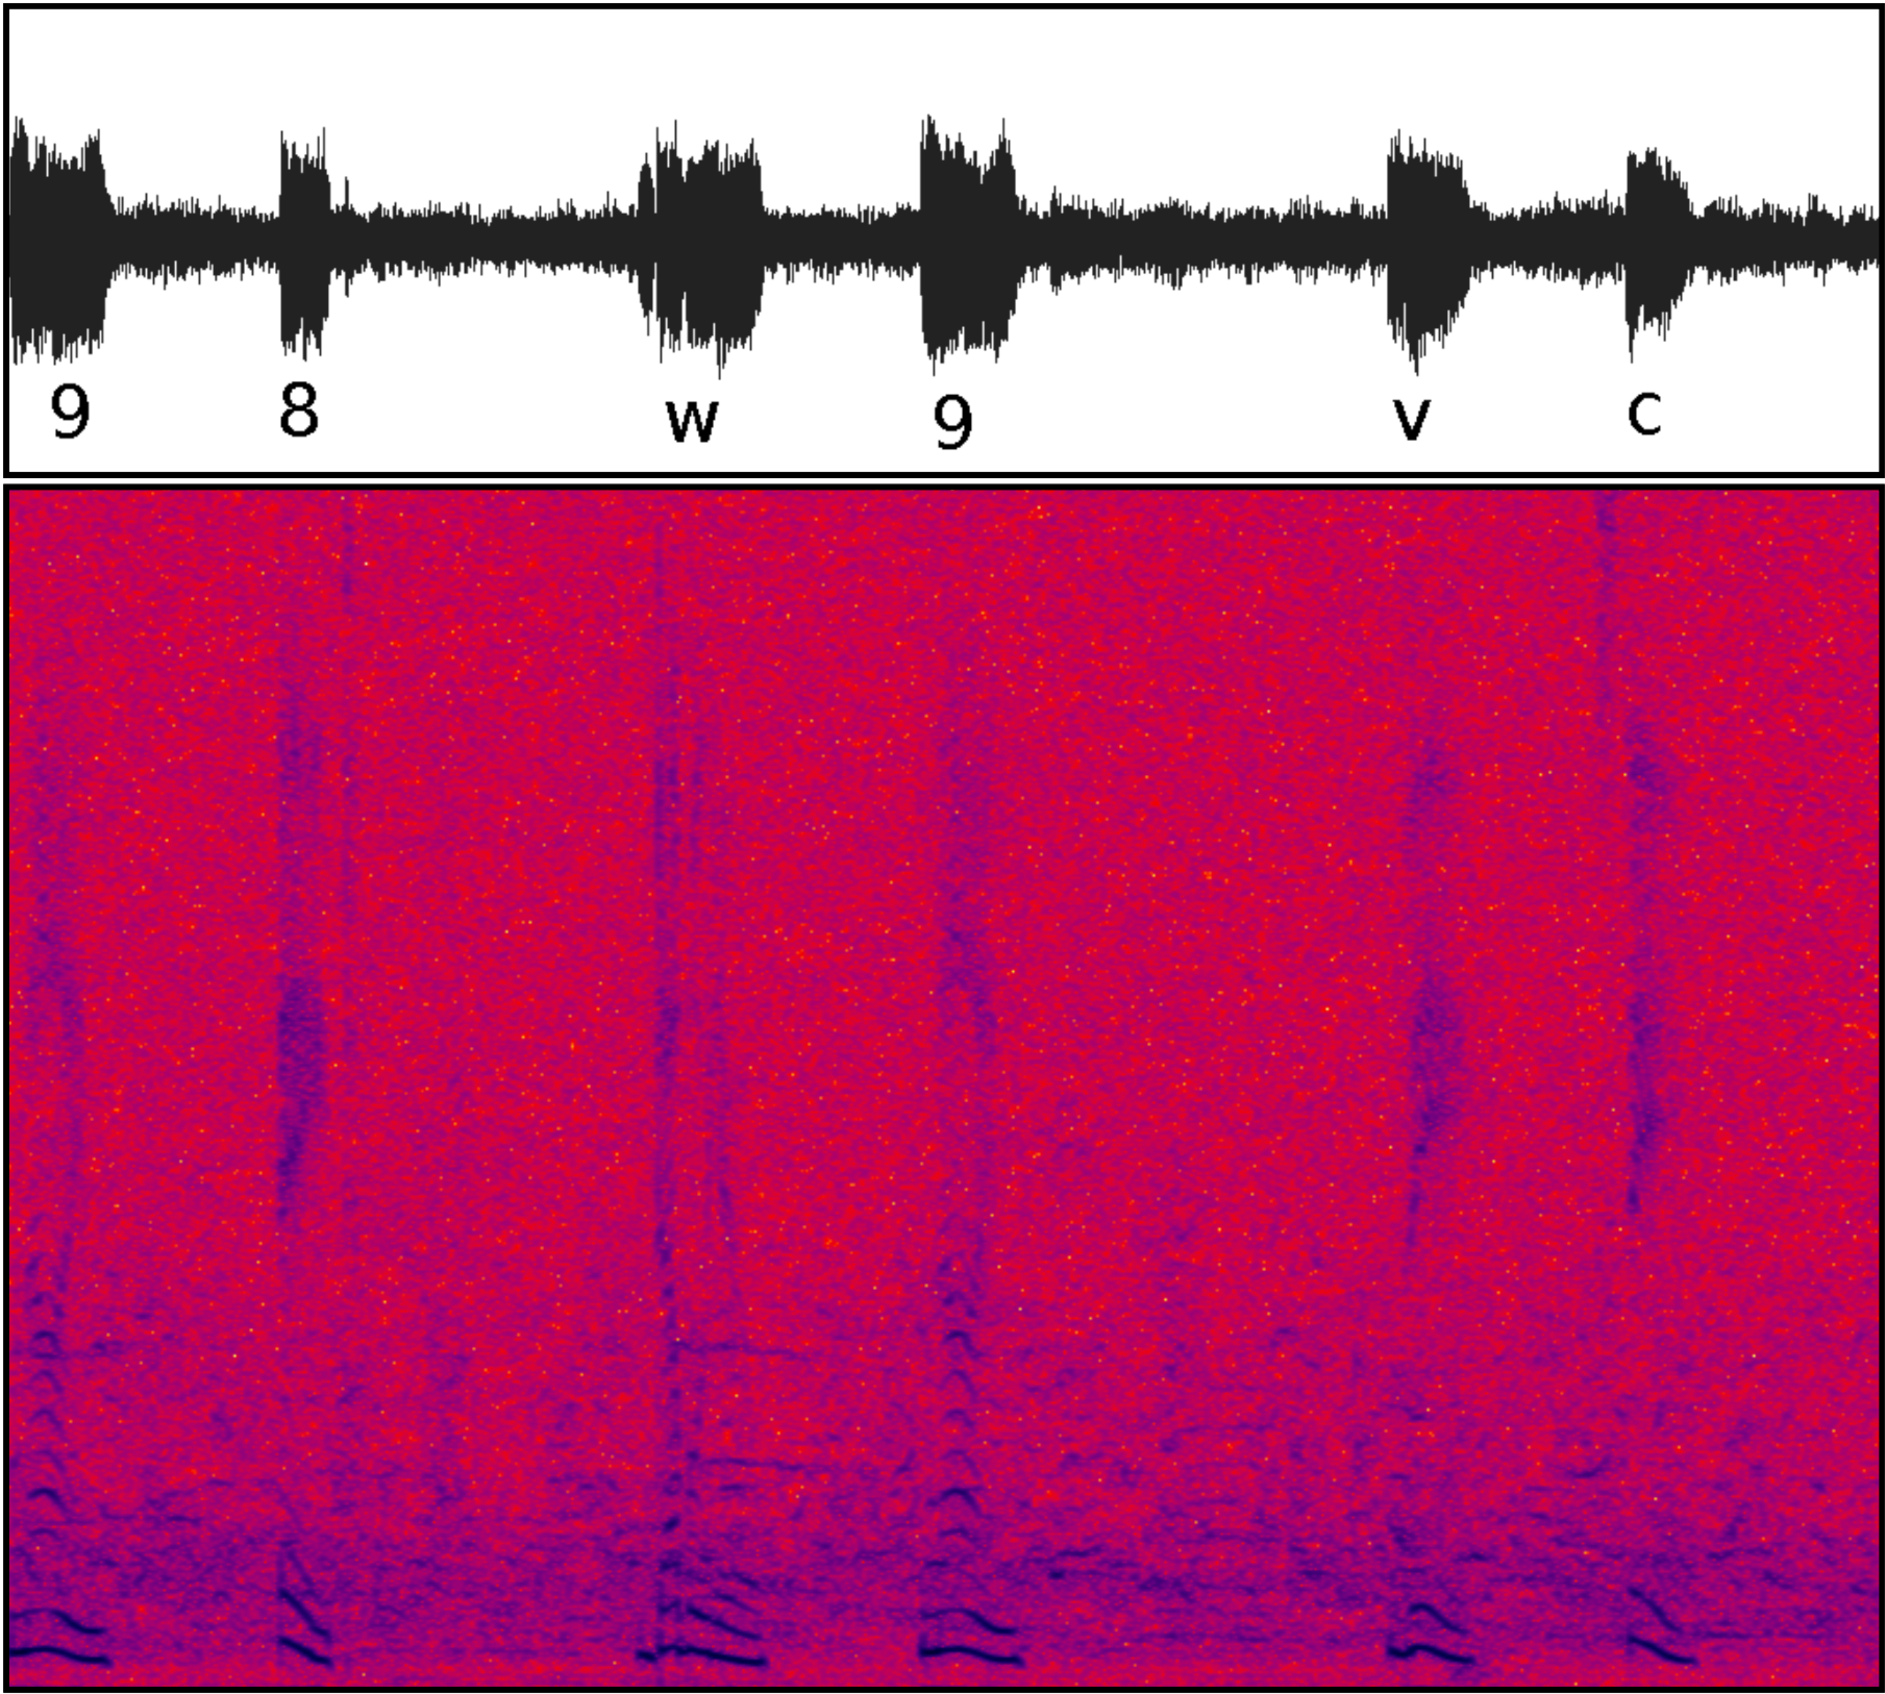
\includegraphics[width=\textwidth]{figures/secure.pdf}
        \caption{Securimage}
        \label{fig:secure}
\end{subfigure}\hspace{0.03\textwidth}
\begin{subfigure}{0.3\textwidth}
        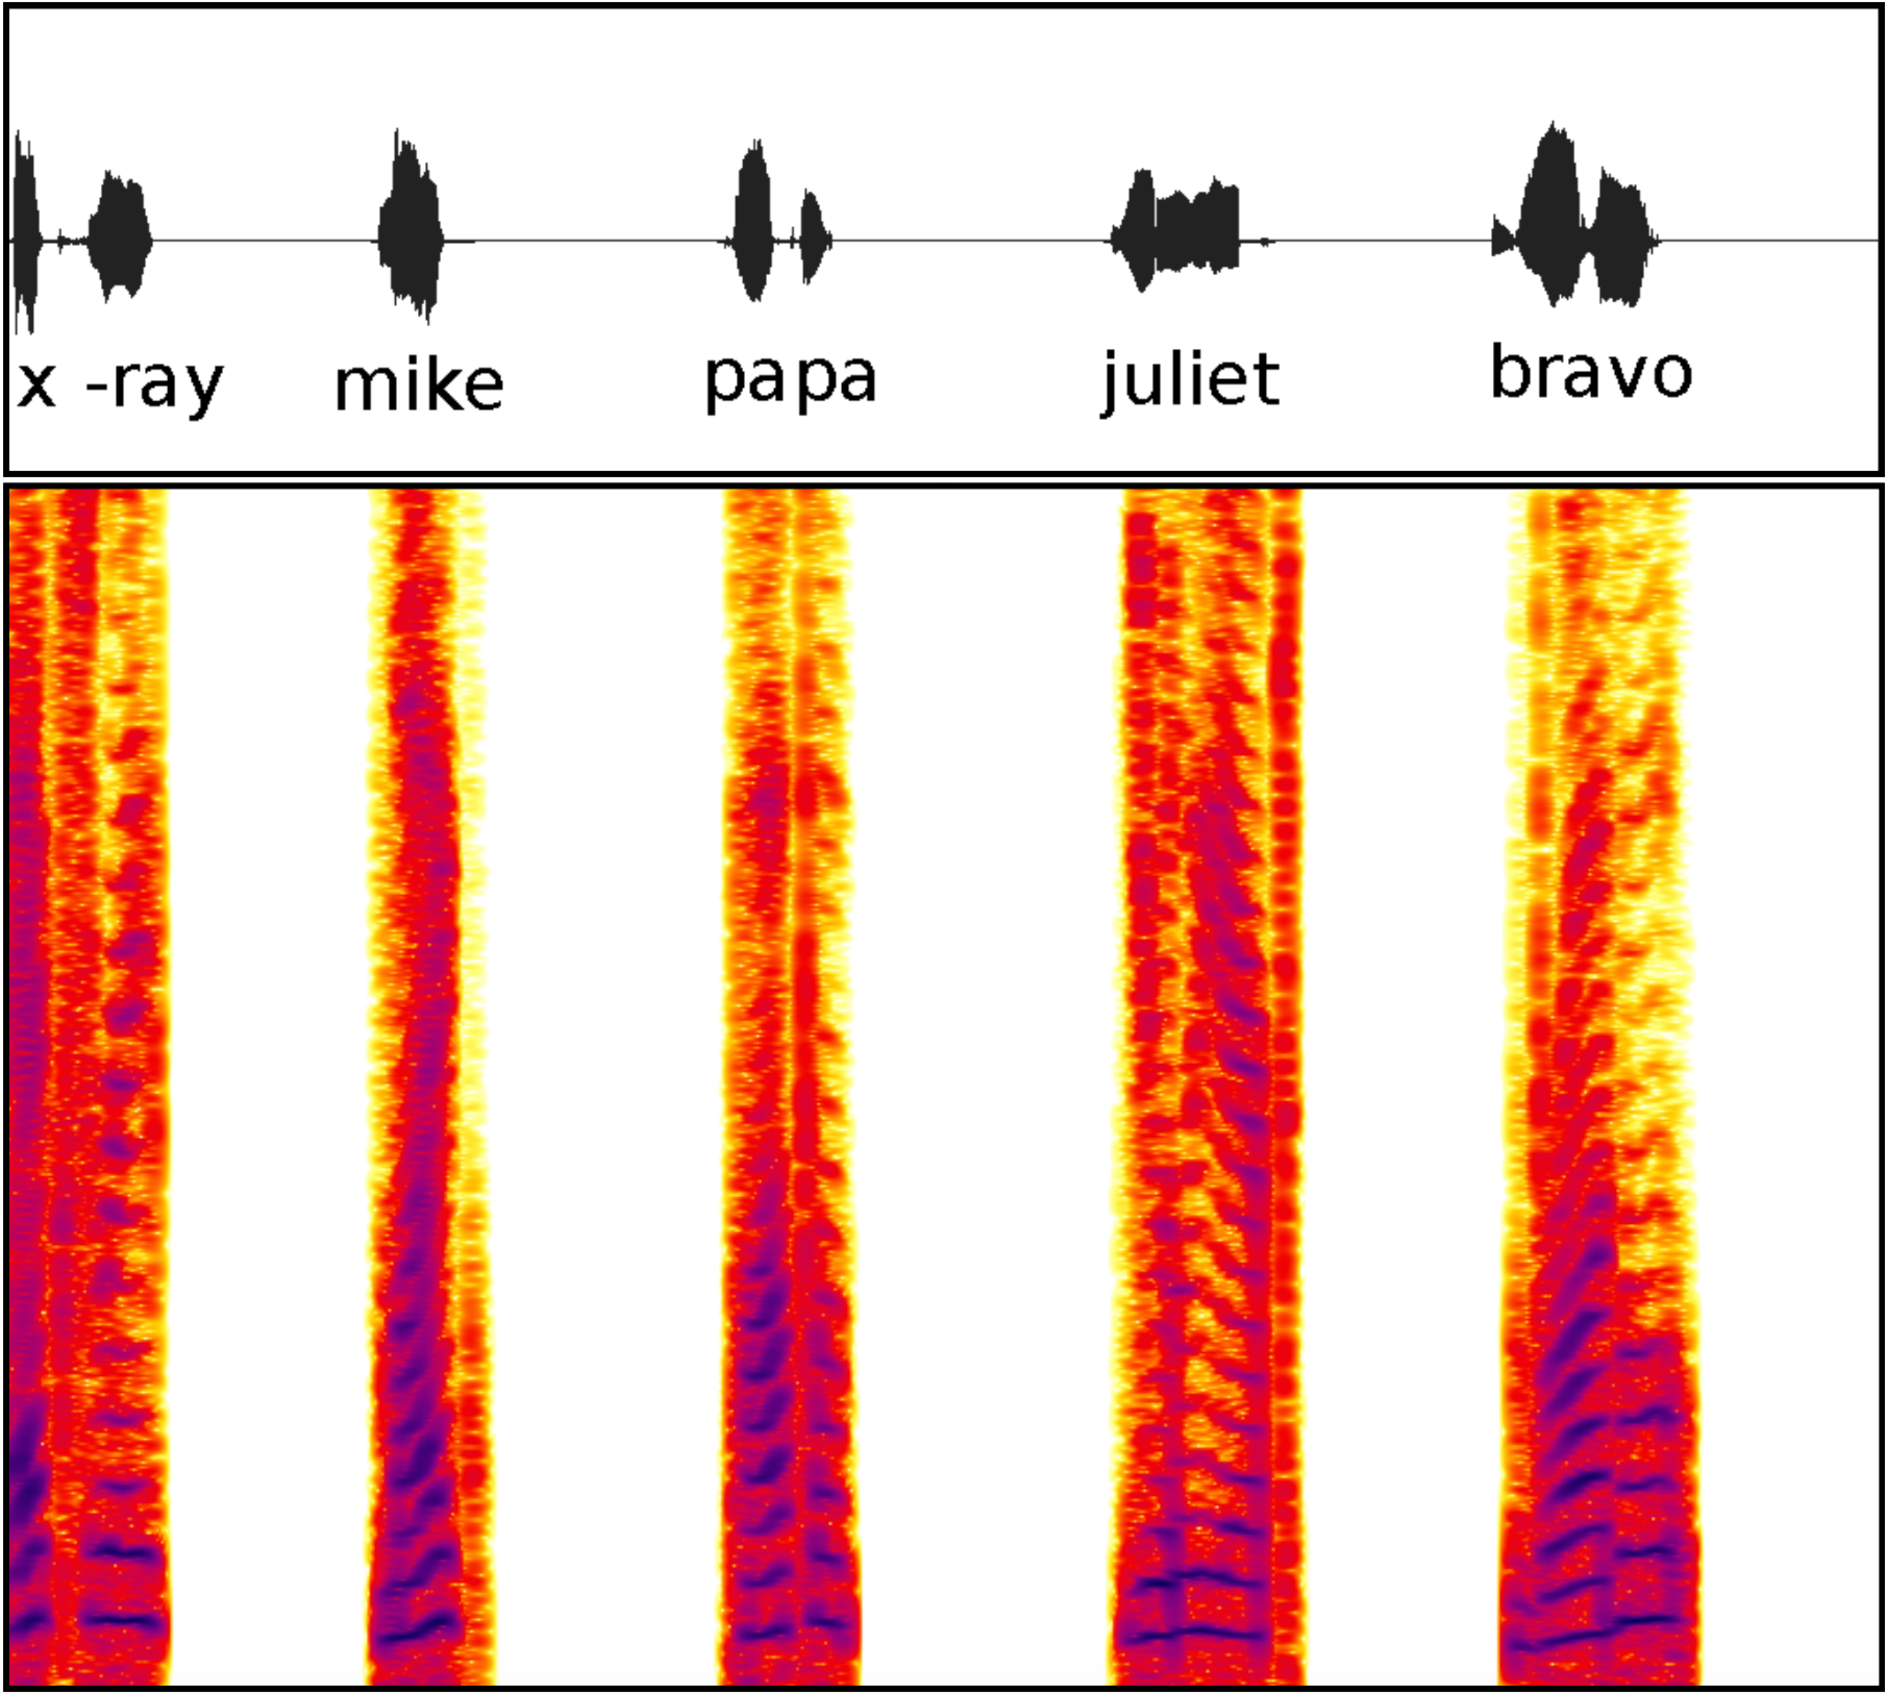
\includegraphics[width=\textwidth]{figures/telerik.pdf}
        \caption{Telerik}
        \label{fig:telerik}
\end{subfigure}
\caption{Waveforms and corresponding spectrograms for a representative sample challenge from every captcha service.}
\label{fig:examples}
\end{figure*}

\subsection{Google \re}
\label{sec:recaptcha}

Google's Recaptcha system, which is the most widely deployed captcha system,
has evolved significantly from its original form, both for adapting to publicized 
attacks (e.g.,~\cite{GoodfellowBIAS13}) and for minimizing the nuisance 
presented to users. While the audio version has not evolved as drastically from its original 
form, during our experiments there was a change in the audio challenges; we 
differentiate between the 2 versions in the remainder of the paper.

%Google provides a demo page for Recaptcha, its state-of-the-art captcha system (the version 2 of Recaptcha), 
%accessible via the following URL (https://www.google.com/\newline recaptcha/api2/demo), for anyone who wants 
%to try out the new captcha system. We used this demo page for all our tests on Recaptcha. The page connects 
%over HTTPS and does not require a login. The page initially loads a widget with a checkbox, which on clicking, 
%shows another widget with the image captcha that loads in a new iframe. The audio captcha challenge appears only 
%after clicking on the headphones-like icon in the bottom of the second widget.

\textbf{Recaptcha v2.0.} The audio challenge provided by the \re system spells out 5 digits
consecutively with little or noise, while the interval between the digits fluctuates. 
Each digit may be spoken out by the same individual (male or female), or multiple 
speakers may be employed. While the challenges do not contain background noise, certain 
spoken digits have a more distorted nature and sound drawn out or slowed down.  %Accents tend to not differ that much.

%The challenge also provides an option for the user to download the .mp3 version of the audio. The recaptcha system provides 
%a margin for error and allows up to 2 incorrect digits out of the 5. We demonstrate how this high margin for error can be 
%leveraged to get an almost 100\% accuracy value. We were able to exploit a security flaw in this system that allowed us to 
%bypass the rate limiting that was in place.
%
%The recaptcha demo page generates a new captcha challenge each time we connect to it. It behaves exactly like the recaptcha 
%v2 widget that is embedded in popular websites such as Quora, BusinessInsider, Twitter, Ticketmaster and many more, as part 
%of their account creation process. This was one of the main reasons why we chose to do our tests with the demo page, instead 
%of any particular website that employs Google's recaptcha. Our results would thus stay valid on any website that has the latest 
%recaptcha widget embedded.

\textbf{Recaptcha v2.1.} This is the latest version of \re that was released after our initial period of experiments (deployed in March 2017).
To offer a more accurate and complete picture of how the system has evolved, we include experiments against both versions.
This version is part of the latest ``Invisible \re'' version which builds upon the ``No Captcha \re'' risk analysis engine attacked in 
previous work~\cite{sivakorn:eurosp16}. This version spells out 10 consecutive digits without background noise, but also includes
recordings of digits that sound distorted.

%\textbf{Recaptcha 1.0} Although still used in many websites, Google has discontinued this version of \re since 2014.
%Furthermore, signing up for \re now will enable the newest version by default. It must be
%noted that the websites that used this version previously did not automatically upgrade to the No 
%captcha Recaptcha version, and remain open to the vulnerabilities that were fixed in the subsequent 
%version. Again, ten digits are spoken in the audio challenge and there is very little or no noise. This 
%version does not enforce any rate limiting unlike the newer versions of \re. The margin for error 
%is again 1 out of the 10 spoken digits. We have obtained \note{X} samples from the authors 
%of~\cite{meutzner2014using} so as to compare the effectiveness of our attack that uses 
%off-the-shelf speech recognition systems against previous studies that used custom
%machine learning classifiers.

\textbf{Automating.} As detailed in previous work~\cite{sivakorn:eurosp16}, \re employs various
safeguards that compliment the captcha challenges and aim to mitigate the extent of automated 
actions.

\emph{Form filling.} \re's analysis engine also detects bots by measuring the time delay between
each text box being filled in for identifying automated actions. To overcome this we introduce 
random delays between each action (the engine also flags bots that maintain a constant delay 
between actions).

\emph{Rate limiting.} One of the safeguards in place aims to throttle automated attacks by limiting 
the amount of captchas that can be solved by a single machine (similar to the token buckets approach proposed by
Elson et al.~\cite{asirra}). In Section~\ref{sec:evaluation} we describe a bug that we identified in the system
that allowed us to bypass this check.

\subsection{Apple}

Apple's captcha is encountered while signing up for a new iCloud account.
Before spelling out the audio challenge,
the voice first says ``Please enter the $n$ numbers that you hear in the textbox provided''. The 
spoken numbers consist of two digits spoken by a single speaker with a synthetic/robotic voice.
Backgorund noise is only present when the numbers are spoken,
and resembles a clamor of children.
The page times out after two minutes of inactivity and a pop up appears for confirmation if the user is 
still in the process of creating the account. 
%Apple does not allow downloading the audio file and is 
%loaded and played via JavaScript and not stored in any cache or temporary storage.

%To obtain the audio file for the challenge, one has to manually open the URL chrome://media-internals 
%on the Google Chrome browser. The Media Internals feature of Chrome displays three things \cite{media}:
%\begin{itemize}
%\item Everything it can dig up from the media stack about active media players. Includes buffered data, 
%    video properties, measured times between events, and a log of events.
%\item Status and volume of active audio streams. These are not yet associated with a particular tab.
%\item Cache activity, including reads from and writes to the media cache.\newline
%\end{itemize}

\textbf{Automating.} Apple has opted for certain design choices that pose obstacles to automated actions,
which we discuss below.

\emph{Obtaining audio.} By deploying their own HTML5 audio player Apple has made it 
difficult to obtain the audio recording, as opposed to other services like \re
that allow a straightforward fetching of the mp3 file. As a workaround, we access 
the browser's media stack\footnote{Through chrome://media-internals.} and obtain the 
audio recording in base64 format.

\emph{Form filling.} Form elements are not accessible via HTML ids/tags; instead we enumerate them 
using XPath (input[@type='text']), and access them according to attribute values.
Furthermore, the system requires mouse interaction for actually accessing an element, otherwise the 
form's validation script will not execute if the answer box has not been ``touched''. We automate this 
process using PyWinAuto~\cite{pywinauto}.
%basically having 
%something like a js framework or html5 template to create the web application GUI makes it slightly more difficult to bot. (very slightly)

%\note{Use user agent spoofing to hide your behaviour.}

\textbf{Pre-processing.} We remove the spoken instructions at the beginning of the audio file
before it is sent to the service.

\begin{table*}[t]
\centering
\caption{Accuracy of different speech recognition services and accents against the audio captcha services we evaluated.}
\begin{tabular}{lccccc}
\toprule
&\multicolumn{5}{c}{\textbf{Speech Recognition Service (Accent)}}\\
\cmidrule{2-6}
\textbf{Captcha Service}& \textbf{Wit}& \textbf{IBM (US)} & \textbf{ IBM (UK)} & \textbf{Google (US)} & \textbf{Google (UK)} \\
\hline
Recaptcha v2.0 & 67.1\% (671/1000) & 95.8\% (958/1000) & 67.2\% (672/1000) & \textbf{98.3\%} (983/1000) & 81.6\% (816/1000) \\
\rowcolor{Gray}
Recaptcha v2.1 & -  & - & -  & \textbf{83.9\%} (1786/2128) & - \\
Apple  & 0\% (0/365)  & 2.3\% (6/260) & 6.8\% (17/251) & 35.8\% (126/352) & \textbf{52.8\%} (143/271) \\
\rowcolor{Gray}
BotDetect  & 1.23\% (11/894)  & 1.38\% (19/138) & 6.67\% (12/180) & \textbf{9.5\%} (102/1067)  & 6.65\% (79/1187) \\
Captchas.net  & 0\% (0/1008) & 1.1\% (9/778)  & 0.3\% (3/1010)  & 2.7\% (16/593) & \textbf{22.3\%} (230/1030) \\
\rowcolor{Gray}
Microsoft Live & 24.7\% (71/287) &  &  & 21.2\$ (28/132)  & 18.6\$ (27/145) \\
Securimage  & 0\% (0/1000)  & 0\% (0/1000) & 0\% (0/1000) & 0.1\% (0/1000) & \textbf{3\%} (30/1000) \\
\rowcolor{Gray}
Telerik  & 21.2\% (142/668)  & \textbf{97\%} (452/466) & 12.9\% (47/364) & 74.2\% (150/202) & 49.3\% (112/217) \\
\bottomrule
\end{tabular}
\label{tab:combinations}
\end{table*}


\subsection{BotDetect}
%BotDetect offers free and paid versions of its captcha system. In the free version, the 
%service has several limitations, like the audio challenge is not fully functional most of 
%the times. There is a 50\% chance that the audio challenge is replaced with an audio file 
%that speaks "Sound Demo". BotDetect offers libraries for integration with .NET, Java, ASP 
%and PHP based websites. The demo page of BotDetect can be accessed here: 
%\url{https://captcha.com/demos/features/captcha-demo.aspx}.

The audio challenge contains the spoken version of the digits and letters shown in the text captcha.
This captcha service offers many customization options during its integration in a website. For instance, 
the number of alphanumeric characters in the challenge can be chosen between
1-13 (the default being a random selection between 4-6). The background noise can be random or selected from one of 
the 10 noise types and the sound type can be customized as well (choice of 8 Bit Mono audio or 16 Bit 
Mono audio). The default demo version that we experimented with contains intermittent electronic noise that 
coincides with the spoken letters.
%We found that this service is used widely, and we encountered it on the Visa status check 
%page of US CEAC website here: https://ceac.state.gov/ceacstattracker/status.aspx \newline

\subsection{Captchas.net}

Captchas.net started in 2004 offers implementation and easy integration for PHP, ASP, Perl, 
Python, JSP and Ruby. It is a free service, but shows a watermark on the images of the text challenges 
which can be removed by subscribing to the paid version. 
The audio challenges employ the NATO phonetic alphabet, and the user has to enter the corresponding letters.
For instance, ``RIPAZH'' would be read out as 'Romeo India Papa Alpha Zulu Hotel' and the user is expected 
to enter the first letter of each uttered word. The audio challenges contain little background noise during the 
spoken words. However, the words themselves are distorted and sound like digitally synthesized speech.

%For both the text and the audio challenges, 
%Captchas.net follows the following method to validate the response:
%
%\begin{itemize}
%\item Both the client server and Captchas.net's server share a common secret key.
%\item The secret key and a random string sent by the client are used to generate the password.
%\item The password is computed by Captchas.net's server to generate the image and by the client server to validate the user's input.
%\end{itemize}


\subsection{Live.com}

Microsoft's Live domain provides access to other Microsoft services, including
 OneDrive, Bing, MSN, Office, Skype, Outlook.com, Xbox Live, etc. The captcha is 
 encountered while registering for a new account. The audio challenge contains random English 
 words. On average they are 5-letter words and 5-7 such words are spoken per challenge, which must be typed by the user.
The words are spoken by 2 different people - one female and one male. The background noise 
is from speakers talking in a foreign language.
%although we found that the number of words spoken out by the female voice are much higher. In our opinion, it provided better accessibility 
%to visually impaired users as they can press '1' on their keyboard to play or repeat the audio challenge 
%and by requesting a new challenge using the button labeled 'New' on the interface, the focus is set to the 
%response box automatically.

\subsection{Securimage}

Securimage is an open source captcha system that has been under active development and maintenance 
since 2005. It offers plugins/modules for major content management systems, with a lot of customization 
options for both image and audio based challenges. For each audio challenge, the system generates a WAV 
file from a corpus of audio files of 26 alphabets (A-Z) and 10 digits (0-9). The digits and alphabets are 
spoken by a single person. The audio is generated by picking 6 word/digit files at random, combining them and adding one 
of the 5 noise files. The default number of digits/characters per challenge is 6, but this can 
be customized while implementing the library. The entire audio recording contains background noise resembling
human clamor.
%Some other customization options are that one can 
%specify a word list for the challenges and using a read-aloud math puzzle that is to be solved 
%by the user.

\subsection{RadCaptcha by Telerik}

RadCaptcha is a captcha service by Telerik that is built especially for ASP.NET 
web applications. 
%RadCaptcha and 90+ other controls are part of UI for ASP.NET AJAX, 
%a comprehensive toolset that take care of the common functionality of a ASP based
%CMS like Sitefinity \cite{radcaptcha}. 
%It is also a part of a feedback form for the 
%HR website of UIC, where we discovered this captcha. It can be seen here: https://www
%.hr.uic.edu/cms/One.aspx?pageId=356957\newline
RadCaptcha's audio challenge contains digits (0-9) and the NATO phonetic alphabet. It is 
spelled out by a single speaker and there is almost no background noise in the audio. 
%The 
%audio is not available to download explicitly, but is present on the DOM of the web page 
%in an <audio> tag, from which the URL of the audio file can be easily grabbed. 
One of the customizations provided by the service is a throttling measure, which requires the form to 
be displayed to the user for a particular number of seconds before an answer will be considered as 
human-submitted. However, this setting is left up to the developer who incorporates the captcha 
service on the target web page.

